\appendix
\section{\appendixname}
\frame{\tableofcontents}

\subsection{KIM}

\begin{frame}{Custo zero nas arestas}
%%%%%%%%%%%%%%%%%%%%%%%%%%%%%%%%%%%%%%%%%%%%%%%%%%%%%%%%%%%%%%%%%%%%%%%%%%%%%%%%%%%
%%%%%%%%%%%%%%%%%%%%%%%%%%%%%%%%%%grafo%%%%%%%%%%%%%%%%%%%%%%%%%%%%%%%%%%%%%%%%%%%5
%%%%%%%%%%%%%%%%%%%%%%%%%%%%%%%%%%%%%%%%%%%%%%%%%%%%%%%%%%%%%%%%%%%%%%%%%%%%%%%%%%%
\begin{figure}
\tikzstyle{vertex}=[circle,fill=black!25,minimum size=15pt,inner sep=0pt]
\tikzstyle{start} = [vertex, fill=red!24]
\tikzstyle{end} = [vertex, fill=red!24]
\tikzstyle{edge} = [draw,thick,-]
\tikzstyle{weight} = [font=\tiny]
\tikzstyle{selected edge} = [draw,line width=2pt,-,red!50]
	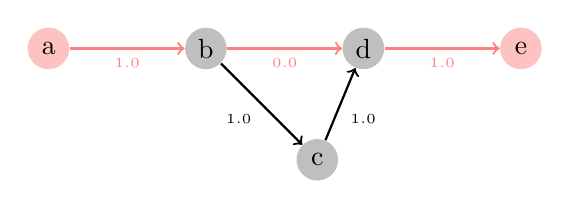
\begin{tikzpicture}[scale=1.8, auto,swap,node distance=2cm]
        \node[start] (a) {a};
        \node[vertex] (b) [right of=a] {b};
        \node[vertex] (c) [below right of=b] {c};
        \node[vertex] (d) [right of=b] {d};
        \node[end] (e) [right of=d] {e};
          
         \path[selected edge] (a) -- node[weight] {$1.0$} (b);
         \path[selected edge] (b) -- node[weight] {$0.0$} (d);
         \path[selected edge] (d) -- node[weight] {$1.0$} (e);
         \path[edge] (b) -- node[weight] {$1.0$} (c);
         \path[edge] (c) -- node[weight] {$1.0$} (d);
   \end{tikzpicture}
\end{figure}
%%%%%%%%%%%%%%%%%%%%%%%%%%%%%%%%%%%%%%%%%%%%%%%%%%%%%%%%%%%%%%%%%%%%%%%%%%%%%
\begin{columns}[b]
 \column{.3\textwidth}
   \onslide<2->
	    {%
\begin{figure}
\tikzstyle{node}=[circle,fill=black!25,minimum size=10pt,inner sep=0pt]
\tikzstyle{root} = [node, fill=red!24]
\tikzstyle{leaf} = [node, fill=red!24]
\tikzstyle{onPath} = [node, fill=red!24]
\tikzstyle{edge} = [draw,thick,->]
\tikzstyle{weight} = [font=\tiny]
\tikzstyle{selected edge} = [draw,thick,->,red!50]
%\tikzstyle{LabelStyle}=[fill=white,sloped]
\begin{tikzpicture}[scale=0.8]
% Set the overall layout of the tree
\tikzstyle{level 1}=[level distance=1.5cm, sibling distance=2.5cm]
\tikzstyle{level 2}=[level distance=1.5cm, sibling distance=2.5cm]
  	\node[root,label=right:{\footnotesize $\epsilon=1$}] (a) {a} [grow=down,->] 
  	    child {
				node[onPath,label=right:{\footnotesize $\epsilon=2$}] (ab) {b}
				child{
						node[onPath,label=right:{\footnotesize $\epsilon=3$}](abd){d} 
						child{
							node[onPath,label=left:{\footnotesize $\epsilon=4$}] (abde) {e}
							edge from parent
							node[left,weight] {1.0}
						}
						child {
							node[node,label=right:\textcolor{red}{\footnotesize $\epsilon=3$}] {c}
							edge from parent
							node[right,weight] {1.0}
	 					}
						edge from parent
						node[left,weight] {0.0}
				}
				edge from parent
				node[left,weight] {1.0}
	 }
	     ;
  	\path[selected edge] (a) -- node[weight] {} (ab);
   \path[selected edge] (ab) -- node[weight] {} (abd);
   \path[selected edge] (abd) -- node[weight] {} (abde);   
	\end{tikzpicture}
	
	\end{figure}
}
 \column{.3\textwidth}
   \onslide<2->
	    {%
\begin{figure}
\tikzstyle{node}=[circle,fill=black!25,minimum size=10pt,inner sep=0pt]
\tikzstyle{root} = [node, fill=red!24]
\tikzstyle{leaf} = [node, fill=red!24]
\tikzstyle{onPath} = [node, fill=red!24]
\tikzstyle{edge} = [draw,thick,->]
\tikzstyle{weight} = [font=\tiny]
\tikzstyle{selected edge} = [draw,thick,->,red!50]
%\tikzstyle{LabelStyle}=[fill=white,sloped]
\begin{tikzpicture}[scale=0.8]
% Set the overall layout of the tree
\tikzstyle{level 1}=[level distance=1.5cm, sibling distance=2.5cm]
\tikzstyle{level 2}=[level distance=1.5cm, sibling distance=2.5cm]
  	\node[root,label=right:{\footnotesize $\zeta=4$}] (e) {e} [grow=up,->] 
  	    child {
				node[onPath,label=right:{\footnotesize $\zeta=3$}] (ed) {d} 
				child{
						node[onPath,label=right:{\footnotesize $\zeta=2$}] (edb) {b}  
						child{
							node[onPath,label=right:{\footnotesize $\zeta=1$}] (edba) {a} 
							edge from parent
							node[right,weight] {1.0}
						}
						child {
							node[node,label=left:\textcolor{red}{\footnotesize $\zeta=2$}] {c}
							edge from parent
							node[left,weight] {1.0}
	 					}
						edge from parent
						node[left,weight] {0.0}
				}
				edge from parent
				node[left,weight] {1.0}
	 }
	     ;
 	\path[selected edge] (e) -- node[weight] {} (ed);
   \path[selected edge] (ed) -- node[weight] {} (edb);
   \path[selected edge] (edb) -- node[weight] {} (edba);
	\end{tikzpicture}
	
	\end{figure}
}
	\column{.4\textwidth}
   \onslide<3->
	    {%
		\begin{center}
		\begin{block}{Problema}
		\begin{itemize}
			\item {\small $\epsilon(c)>\zeta(c)$}
			\item {\small N�o consegue gerar o caminho $\seq{a,b,c,d,e}$} 
		\end{itemize}
		\end{block}

		\end{center}
	}
\end{columns}
\end{frame}

\begin{frame}{$P_a$}
\only<1>{
Na figura temos os caminhos $P_j$ e $P_k$, $1<=j<k$ onde $P_j$ � pai de $P_k$ e que compartilham o prefixo $\seq{s,\ldots,u}$
diferenciando-se a partir de $u$.
}
\only<2>{
Esquema dos caminhos na parti��o $P_a$.
}
\begin{figure}[c]
\tikzstyle{node}=[circle,fill=black!25,minimum size=10pt,inner sep=0pt]
\tikzstyle{root} = [node, fill=red!24]
\tikzstyle{leaf} = [node, fill=red!24]
\tikzstyle{deviation} = [node, fill=blue]
\tikzstyle{onPath} = [node, dashed,fill=red!24]
\tikzstyle{edge} = [draw,thick,->]
\tikzstyle{unknown} = [dashed,thick,->]
\tikzstyle{novos} = [node, fill=red!50]
\tikzstyle{weight} = [font=\tiny]
\tikzstyle{selected edge} = [draw,thick,->,red!50]
%\tikzstyle{LabelStyle}=[fill=white,sloped]
\only<1>{
\begin{tikzpicture}[scale=1]
% Set the overall layout of the tree
\tikzstyle{level 1}=[level distance=1.5cm, sibling distance=2.5cm]
\tikzstyle{level 2}=[level distance=1.5cm, sibling distance=2.5cm]
\node[root,label=right:{s}] {}
child {
				node[deviation,label=right:{u}] {}
				child[->,solid] {
						node[node] {a}
						child[->,dashed]{
							node[leaf] {$t_j$}
						}
				}
				child[->,solid] {
					node[node] {b}
						child[grow=down,dashed]{
							node[leaf] {$t_{k}$} 
						}
				}
				edge from parent[dashed]
};
\end{tikzpicture}
}
\only<2> 
{
\begin{tikzpicture}[scale=1]
% Set the overall layout of the tree
\tikzstyle{level 1}=[level distance=1.5cm, sibling distance=2.5cm]
\tikzstyle{level 2}=[level distance=1.5cm, sibling distance=2.5cm]
\node[root,label=right:{s}] (s) {}
child {
				node[deviation,label=right:{u}] {}
				child[->,solid] {
						node[node] {a}
						child[->,dashed]{
							node[leaf] {$t_j$}
						}
				}
				child[->,solid] {
					node[node] {b}
						child[sibling distance=10mm,level distance=1cm,dashed,->,line width=2pt]{node[novos]{}}
						child[sibling distance=10mm,level distance=1cm,dashed,->]{
							child[dashed,line width=2pt]{node[novos]{}}
							child[line width=2pt]{node[novos]{}}
							child[level distance=1.5cm,grow=down]{
								node[leaf] {$t_{k}$} 
							}
							child[line width=2pt]{node[novos]{}}
							child[line width=2pt]{node[novos]{}}
						}
						child[sibling distance=10mm,level distance=1cm,dashed,->,line width=2pt]{node[novos]{}}
					}
				edge from parent[dashed]
};
\end{tikzpicture}

}

\end{figure}
\end{frame}

\begin{frame}{$P_b$}
\begin{figure}
\tikzstyle{node}=[circle,fill=black!25,minimum size=10pt,inner sep=0pt]
\tikzstyle{root} = [node, fill=red!24]
\tikzstyle{leaf} = [node, fill=red!24]
\tikzstyle{novos} = [node, fill=red!70]
\tikzstyle{deviation} = [node, fill=blue]
\tikzstyle{onPath} = [node, dashed,fill=red!24]
\tikzstyle{edge} = [draw,thick,->]
\tikzstyle{unknown} = [dashed,thick,->]
\tikzstyle{filhos} = [node,fill=green!50]
\tikzstyle{weight} = [font=\tiny]
\tikzstyle{selected edge} = [draw,thick,->,red!50]
%\tikzstyle{LabelStyle}=[fill=white,sloped]
\only<1>{
\begin{tikzpicture}[scale=1]
% Set the overall layout of the tree
\tikzstyle{level 1}=[level distance=1.5cm, sibling distance=2.5cm]
\tikzstyle{level 2}=[level distance=1cm, sibling distance=2cm]
\node[root,label=right:{s}] {}
child {
				node[deviation,label=right:{u}] {}
				child[->,dashed]{node[filhos]{}}
				child[->,dashed] {
						child[->,dashed]{node[filhos]{}}
						child[->,dashed,grow=down]{
							child[->,dashed]{
													node[filhos]{}
							}
							child[->,dashed,grow=down]{
													child[->,dashed]{
																			node[filhos]{}
													}
													child[->,dashed,grow=down]{
																			node[leaf] {$t_j$}
													}
							}
						}
				}
				child[->,solid] {
					node[node] {b}
						child[grow=down,dashed]{
							node[leaf] {$t_{k}$} 
						}
				}
				edge from parent[dashed]
};
\end{tikzpicture}
}
\only<2>{
\begin{tikzpicture}[scale=1]
% Set the overall layout of the tree
\tikzstyle{level 1}=[level distance=1.5cm, sibling distance=2.5cm]
\tikzstyle{level 2}=[level distance=1cm, sibling distance=2cm]
\node[root,label=right:{s}] {}
child {
				node[deviation,label=right:{u}] {}
				child[->,dashed]{node[filhos]{}}
				child[->,dashed] {
						node[deviation,label=right:{v}] {}
						child[->,dashed]{node[filhos]{$i_l$}}
						child[->,dashed,grow=down]{
							child[->,dashed]{
													node[filhos]{}
							}
							child[->,dashed,grow=down]{
													child[->,dashed]{
																			node[filhos]{}
													}
													child[->,dashed,grow=down]{
																			node[leaf] {$i_j$}
													}
							}
						}
				}
				child[->,solid] {
					node[node] {b}
						child[grow=down,dashed]{
							node[leaf] {$i_{k}$} 
						}
				}
				edge from parent[dashed]
};
\end{tikzpicture}
}
\only<3>{
\begin{tikzpicture}[scale=1]
% Set the overall layout of the tree
\tikzstyle{level 1}=[level distance=1.5cm, sibling distance=2.5cm]
\tikzstyle{level 2}=[level distance=1cm, sibling distance=2cm]
\node[root,label=right:{s}] {}
child {
				node[deviation,label=right:{u}] {}
				child[->,dashed,line width=2pt]{node[novos]{}}
				child[->,dashed]{node[filhos]{}}
				child[grow=down]{
					child[->,dashed,line width=2pt]{node[novos]{}}
					child[grow=down,level distance=5mm]{
						child[level distance=10mm,grow=south east,->,dashed,line width=2pt]{node[novos]{}}
						child[level distance=15mm,->,dashed,grow=down] {
								node[deviation,label=right:{v}] {}
								child[level distance=10mm,->,dashed]{node[leaf]{$t_l$}}
								child[level distance=10mm,->,dashed,grow=down]{
										node[leaf] {$t_j$}
								}
						}
					}
				}
				child[->,solid] {
					node[node] {b}
						child[grow=down,dashed]{
							node[leaf] {$t_k$} 
						}
				}
				edge from parent[dashed]
};
\end{tikzpicture}
}
\end{figure}
\end{frame}

\begin{frame}{$P_c$}
\begin{figure}
\tikzstyle{node}=[circle,fill=black!25,minimum size=10pt,inner sep=0pt]
\tikzstyle{root} = [node, fill=red!24]
\tikzstyle{leaf} = [node, fill=red!24]
\tikzstyle{novos} = [node, fill=red!70]
\tikzstyle{deviation} = [node, fill=blue]
\tikzstyle{onPath} = [node, dashed,fill=red!24]
\tikzstyle{edge} = [draw,thick,->]
\tikzstyle{unknown} = [dashed,thick,->]
\tikzstyle{filhos} = [node,fill=green!50]
\tikzstyle{weight} = [font=\tiny]
\tikzstyle{selected edge} = [draw,thick,->,red!50]
%\tikzstyle{LabelStyle}=[fill=white,sloped]
\only<1>{
\begin{tikzpicture}[scale=1]
% Set the overall layout of the tree
\tikzstyle{level 1}=[level distance=5mm, sibling distance=2cm]
\tikzstyle{level 2}=[level distance=5mm, sibling distance=2cm]
\node[root,label=right:{s}] {}
child {
	child[->,dashed]{node[filhos]{}}
		child[-,dashed,grow=down]{
			child[-,dashed]{
				node{$\ldots$} edge from parent[draw=none]
			}
			child[->,dashed,grow=down]{
				child[->,dashed]{
					node[filhos]{}
				}
				child[level distance=1.5cm,->,dashed,grow=down]{	
					node[deviation,label=right:{u}] {}
					child[grow=down,dashed]{
						node[leaf] {$t_{k}$} 
					}
					child{
						node[leaf] {$t_j$}
					}
				}
			}
		}
	edge from parent[dashed]
};
\end{tikzpicture}
}
\only<2>{
\begin{tikzpicture}[scale=1]
% Set the overall layout of the tree
\tikzstyle{level 1}=[level distance=5mm, sibling distance=2cm]
\tikzstyle{level 2}=[level distance=5mm, sibling distance=2cm]
\node[root,label=right:{s}] {}
child {
	child[->,dashed]{node[leaf]{}}
		child[-,dashed,grow=down]{
			child[-,dashed]{
				node{$\ldots$} edge from parent[draw=none]
			}
			child[->,dashed,grow=down]{
				node[deviation,label=right:{v}]{}
				child[->,dashed]{
					node[filhos]{$t_l$}
				}
				child[level distance=1.5cm,->,dashed,grow=down]{	
					node[deviation,label=right:{u}] {}
					child[grow=down,dashed]{
						node[leaf] {$t_{k}$} 
					}
					child{
						node[leaf] {$t_j$}
					}
				}
			}
		}
	edge from parent[dashed]
};
\end{tikzpicture}
}
\only<3>{
\begin{tikzpicture}[scale=1]
% Set the overall layout of the tree
\tikzstyle{level 1}=[level distance=5mm, sibling distance=2cm]
\tikzstyle{level 2}=[level distance=5mm, sibling distance=2cm]
\node[root,label=right:{s}] {}
child {
		child[-,dashed,grow=down]{
			child[->,dashed,grow=down]{
				node[deviation,label=right:{v}]{}
				child[->,dashed,line width=2pt]{
					node[novos]{}
				}
				child[-,grow=down]{
					child[->,line width=2pt]{node[novos]{}}
					child[-,grow=down]{
						child{node{$\ldots$} edge from parent[draw=none]}
						child[-,grow=down]{
							child[->,line width=2pt]{node[novos]{}}
							child[level distance=1.5cm,->,dashed,grow=down]{	
								node[deviation,label=right:{u}] {}
								child[grow=down,dashed]{
									node[leaf] {$t_{k}$} 
								}
								child{
									node[leaf] {$t_j$}
								}
							}
						}
					}
				}
				child[->,dashed]{
					node[filhos]{$t_l$}
				}
			}
		}
	edge from parent[dashed]
};
\end{tikzpicture}
}
\end{figure}
\end{frame}

\subsection{�rvore dos prefixos}
\begin{frame}{Defini��o}
\framesubtitle{\textbf{$\Qcal,(N,E),f,V(\Qcal),A(\Qcal)$}}
\begin{itemize}
	\only<1>{
        \item $\Qcal$: uma cole��o de caminhos
        \begin{columns}
          \column{.3\textwidth}
        \begin{block}{Caminhos}
            {$\seq{s,a,i,t}$} \\
            {$\seq{s,b,f,l,t}$} \\
            {$\seq{s,b,g,l,t}$} \\
            {$\seq{s,b,h,l,t}$} \\
            {$\seq{s,b,h,i,t}$} \\
            {$\seq{s,a,i,h,l,t}$}
        \end{block}
        \end{columns}
        \mbox{} \\
        \mbox{} \\
        \mbox{} \\
     }
	\only<2>{
        \item $(N,E)$: uma arboresc�ncia
        \begin{center}
        \begin{tikzpicture}[auto,thick]
          \tikzstyle{node}=%
          [%
            minimum size=10pt,%
            inner sep=0pt,%
            outer sep=0pt,%
            ball color=example text.fg,%
            circle%
          ]

          \node [node] {} [->]
            child {node [node] {} edge from parent node[swap]{a}}
            child {node [node] {} edge from parent node{e}}
            child {node [node] {} 
                child {node [node] {} edge from parent node{c}}
                edge from parent node{b}
            };
        \end{tikzpicture}
        \end{center}
        \begin{itemize}
        \item Grafo ac�clico $(N,E)$ 
        \item $|N| = |E| + 1$ 
        \item \defi{raiz}
        \end{itemize}
        Todo v�rtice, exceto a \defi{raiz}, � ponta final de exatamente um arco.
        }
	\only<3>{
        \item $f$: uma \defi{fun��o r�tulo} 
  \begin{block}{}
	\textbf{Associa n�s e arestas do grafo aos n�s e arestas da �rvore de prefixos.}
  \end{block}
  Se \begin{eqnarray*}
  R=\seq{u_{0}, e_{1}, u_{1}, \ldots, e_{t}, u_{t}}
  \end{eqnarray*}
  for um caminho em  $(N,E)$, ent�o
  \begin{eqnarray*}
  f(R):=\seq{f(u_{0}), f(e_{1}), f(u_{1}), \ldots, f(e_{t}), f(u_{t})}
  \end{eqnarray*}
  ser� uma seq��ncia de v�rtices e arcos dos caminhos em $\Qcal$.
        \mbox{} \\
        \mbox{} \\
        \mbox{} \\
        \mbox{} \\
        \mbox{} \\
        }
        \only<1>{
	\item $V(\Qcal)$: conjunto de v�rtices
	\item $A(\Qcal)$: conjunto de arcos
        }
\end{itemize}
\end{frame}

%Seja $(N,E)$ uma arboresc�ncia e  
%$f$ uma \defi{fun��o r�tulo} que associa a cada n� em 
%$N$ um v�rtice em $V(\Qcal)$ e a
%cada arco em $E$ um arco em $A(\Qcal)$. 

%\begin{frame}{Defini��o}
%$(N,E,f)$ � \defi{�rvore dos prefixos} de $\Qcal$ se 
%\begin{itemize}
%\item para cada caminho $R$ em $(N,E)$ com in�cio na
%      raiz, $f(R)$ for prefixo de algum caminho em $\Qcal$; e
%\item para cada prefixo $Q$ de algum caminho em $\Qcal$
%      existir um caminho $R$ em $(N,E)$ com in�cio na
%      raiz tal que $f(R)=Q$; e
%\item o caminho $R$ do item anterior for �nico. 
%\end{itemize}
%\end{frame}

